\documentclass{article}

\usepackage{booktabs}
\usepackage{tabularx}
\usepackage{caption}
\usepackage{bookmark}
\usepackage{enumitem}
\usepackage{hyperref}
\usepackage{graphicx}

% From: https://tex.stackexchange.com/questions/438876/how-to-cross-reference-text-with-a-custom-label-reference-text
\makeatletter
\newcommand{\labeltext}[3][]{%
    \@bsphack%
    \csname phantomsection\endcsname% in case hyperref is used
    \def\tst{#1}%
    \def\labelmarkup{\emph}% How to markup the label itself
    %\def\refmarkup{\labelmarkup}% How to markup the reference
    \def\refmarkup{}%
    \ifx\tst\empty\def\@currentlabel{\refmarkup{#2}}{\label{#3}}%
    \else\def\@currentlabel{\refmarkup{#1}}{\label{#3}}\fi%
    \@esphack%
    \labelmarkup{#2}% visible printed text.
}
\makeatother

\title{Software Requirements Specification: Realm\\\progname}

\author{\authname}

\date{}

%% Comments

\usepackage{color}

\newif\ifcomments\commentstrue %displays comments
%\newif\ifcomments\commentsfalse %so that comments do not display

\ifcomments
\newcommand{\authornote}[3]{\textcolor{#1}{[#3 ---#2]}}
\newcommand{\todo}[1]{\textcolor{red}{[TODO: #1]}}
\else
\newcommand{\authornote}[3]{}
\newcommand{\todo}[1]{}
\fi

\newcommand{\wss}[1]{\authornote{blue}{SS}{#1}} 
\newcommand{\plt}[1]{\authornote{magenta}{TPLT}{#1}} %For explanation of the template
\newcommand{\an}[1]{\authornote{cyan}{Author}{#1}}

%% Common Parts

\newcommand{\progname}{Software Engineering} % PUT YOUR PROGRAM NAME HERE
\newcommand{\authname}{Team \#13, ARC
    \\ Avanish, Ahluwalia
    \\ Russell, Davidson
    \\ Rafey, Malik
    \\ Abdul, Zulfiqar} % AUTHOR NAMES                  

\usepackage{hyperref}
    \hypersetup{colorlinks=true, linkcolor=blue, citecolor=blue, filecolor=blue,
                urlcolor=blue, unicode=false}
    \urlstyle{same}
                                


\begin{document}

\maketitle

\newpage{}

\tableofcontents

\addcontentsline{toc}{section}{Revision History}
\section*{Revision History}

\begin{table}[hp]
    \caption{Revision History} \label{rev_history_table}
    \begin{tabularx}{\textwidth}{p{3cm}p{2cm}X}
        \toprule {\textbf{Date}} & {\textbf{Version}} & {\textbf{Notes}} \\
        \midrule
        2024-10-11 & 1.0 & Initial SRS \\
        \bottomrule
    \end{tabularx}
\end{table}

\section{Introduction}

\wss{This section should provide an overview of the entire document}
\subsection{Document Purpose}

\wss{Describe the purpose of the SRS and its intended audience.}

\subsection{Product Scope}

\wss{Identify the product whose software requirements are specified in this document, including the revision or release number. Explain what the product that is covered by this SRS will do, particularly if this SRS describes only part of the system or a single subsystem. Provide a short description of the software being specified and its purpose, including relevant benefits, objectives, and goals. Relate the software to corporate goals or business strategies. If a separate vision and scope document is available, refer to it rather than duplicating its contents here.}

\subsection{Definitions, Acronyms and Abbreviations}
\label{sub:def_acr_abb}

\begin{itemize}
    \item \labeltext{AR object}{def:ar_obj}: A 2D/3D projection of an entity.
    \item \labeltext{Users}{def:user}: A term for anyone who uses the app.
    \item \labeltext{Organization users}{def:org_user}: Users who belong to an organization that has the ability to create tours. They are affiliated with a particular approved organization who have the ability to modify tours within their organization’s domain.
    \item \labeltext{General users}{def:gen_user}: Users that can access most of the app functionalities except creating tours.
    \item \labeltext{Admins}{def:admin}: People who have access to nothing else but the admin interface within the app.
    \item \labeltext{AR object clusters}{def:ar_obj_cls}: A group of AR objects present within a confined area.
\end{itemize}

\subsection{References}
\label{sub:references}

\wss{List any other documents or Web addresses to which this SRS refers. These may include user interface style guides, contracts, standards, system requirements specifications, use case documents, or a vision and scope document. Provide enough information so that the reader could access a copy of each reference, including title, author, version number, date, and source or location.}

\begingroup
\raggedright
\bibliography{ref}
\endgroup
\bibliographystyle{ieeetr}

\subsection{Document Overview}

\wss{Describe what the rest of the document contains and how it is organized.}

\section{Product Overview}

\wss{This section should describe the general factors that affect the product and its requirements. This section does not state specific requirements. Instead, it provides a background for those requirements, which are defined in detail in Section 3, and makes them easier to understand.}
\subsection{Product Perspective}

\wss{Describe the context and origin of the product being specified in this SRS. For example, state whether this product is a follow-on member of a product family, a replacement for certain existing systems, or a new, self-contained product. If the SRS defines a component of a larger system, relate the requirements of the larger system to the functionality of this software and identify interfaces between the two. A simple diagram that shows the major components of the overall system, subsystem interconnections, and external interfaces can be helpful.}

\subsection{Product Functions}

\wss{Summarize the major functions the product must perform or must let the user perform. Details will be provided in Section 3, so only a high level summary (such as a bullet list) is needed here. Organize the functions to make them understandable to any reader of the SRS. A picture of the major groups of related requirements and how they relate, such as a top level data flow diagram or object class diagram, is often effective.}

\subsection{Product Constraints}
\wss{
    This subsection should provide a general description of any other items that will limit the developer's options. These may include:
    \begin{itemize}
        \item Interfaces to users, other applications or hardware.
        \item Quality of service constraints.
        \item Standards compliance.
        \item Constraints around design or implementation.
    \end{itemize}
}

\begin{itemize}
    \item \textbf{Interfaces to Users}: The platform must be compatible with both Android and iOS devices, meaning the design must accommodate different screen sizes and operating system guidelines. Additionally, the app requires user-friendly interfaces for interacting with AR objects and managing sub-realms.

    \item \textbf{Hardware Constraints}: The app depends on mobile devices with AR capabilities (e.g., cameras, GPS, accelerometers). Users with older or less powerful devices might experience limited functionality or performance issues.

    \item \textbf{Quality of Service}: Realm needs to have a smooth interaction, with little to no lag. It must also handle multiple users within a shared AR space (sub-realm).

    \item \textbf{Standards Compliance}: The app has to comply with relevant privacy laws and app store requirements for both Android and iOS.

    \item \textbf{Design and Implementation Constraints}: The app needs to provide cloud storage for AR objects and user data, and its design should allow for easy scalability as the user base grows. Additionally, the AR features and general app use should be intuitive and easy to use for users.

    \item \textbf{Budget Constraints}: The project has a maximum budget of \$750.
\end{itemize}

\subsection{User Characteristics}

\wss{Identify the various user classes that you anticipate will use this product. User classes may be differentiated based on frequency of use, subset of product functions used, technical expertise, security or privilege levels, educational level, or experience. Describe the pertinent characteristics of each user class. Certain requirements may pertain only to certain user classes. Distinguish the most important user classes for this product from those who are less important to satisfy.}

\subsection{Assumptions and Dependencies}

\wss{List any assumed factors (as opposed to known facts) that could affect the requirements stated in the SRS. These could include third-party or commercial components that you plan to use, issues around the development or operating environment, or constraints. The project could be affected if these assumptions are incorrect, are not shared, or change. Also identify any dependencies the project has on external factors, such as software components that you intend to reuse from another project, unless they are already documented elsewhere (for example, in the vision and scope document or the project plan).}

\begin{itemize}
    \item User has used a mobile app before
    \item User has internet access
    \item User device can provide GPS location services
    \item User device has a camera
    \item User device utilizes either Android or IOS operating systems
\end{itemize}

\subsection{Apportioning of Requirements}

\wss{Apportion the software requirements to software elements. For requirements that will require implementation over multiple software elements, or when allocation to a software element is initially undefined, this should be so stated. A cross reference table by function and software element should be used to summarize the apportioning.\\}

\wss{Identify requirements that may be delayed until future versions of the system (e.g., blocks and/or increments).}

\begin{table}[]
    \caption{Apportioning of Requirements}
    \label{tab:apportioning_table}
    \centering
    \begin{tabular}{lcc}
        \toprule
            \textbf{Function} & \textbf{Priority} & \textbf{Dates} \\
        \hline \hline
    Object Creation          & 1 & \multirow{2}{*}{2024-11-11} \\
    AR Object Interaction    & 1 &                             \\ \hline
    Tour Management          & 2 & \multirow{3}{*}{2025-12-01} \\
    Touring                  & 2 & \\
    Social Interaction       & 2 &                             \\
    Reporting and Moderation & 2 & \multirow{4}{*}{2025-01-15} \\ \hline
    User Profile Management  & 3 &                             \\
    Managing Settings        & 3 &                             \\
    Tutorial                 & 3 &                             \\
        \hline
    \end{tabular}
\end{table}

\section{Requirements}
\wss{
    This section specifies the software product's requirements. Specify all of the software requirements to a level of detail sufficient to enable designers to design a software system to satisfy those requirements, and to enable testers to test that the software system satisfies those requirements.
    The specific requirements should:
    \begin{itemize}
        \item Be uniquely identifiable.
        \item State the subject of the requirement (e.g., system, software, etc.) and what shall be done.
        \item Optionally state the conditions and constraints, if any.
        \item Describe every input (stimulus) into the software system, every output (response) from the software system, and all functions performed by the software system in response to an input or in support of an output.
        \item Be verifiable (e.g., the requirement realization can be proven to the customer's satisfaction)
        \item Conform to agreed upon syntax, keywords, and terms.
    \end{itemize}
}

\subsection{External Interfaces}
\wss{
    This subsection defines all the inputs into and outputs requirements of the software system. Each interface defined may include the following content:
    \begin{itemize}
        \item Name of item
        \item Source of input or destination of output
        \item Valid range, accuracy, and/or tolerance
        \item Units of measure
        \item Timing
        \item Relationships to other inputs/outputs
        \item Screen formats/organization
        \item Window formats/organization
        \item Data formats
        \item Command formats
        \item End messages
    \end{itemize}
}
\subsubsection{User interfaces}

\wss{Define the software components for which a user interface is needed. Describe the logical characteristics of each interface between the software product and the users. This may include sample screen images, any GUI standards or product family style guides that are to be followed, screen layout constraints, standard buttons and functions (e.g., help) that will appear on every screen, keyboard shortcuts, error message display standards, and so on. Details of the user interface design should be documented in a separate user interface specification.}

\wss{Could be further divided into Usability and Convenience requirements.}

\subsubsection{Hardware interfaces}

\wss{Describe the logical and physical characteristics of each interface between the software product and the hardware components of the system. This may include the supported device types, the nature of the data and control interactions between the software and the hardware, and communication protocols to be used.}

\subsubsection{Software interfaces}

\wss{Describe the connections between this product and other specific software components (name and version), including databases, operating systems, tools, libraries, and integrated commercial components. Identify the data items or messages coming into the system and going out and describe the purpose of each. Describe the services needed and the nature of communications. Refer to documents that describe detailed application programming interface protocols. Identify data that will be shared across software components. If the data sharing mechanism must be implemented in a specific way (for example, use of a global data area in a multitasking operating system), specify this as an implementation constraint.}

\subsection{Functional}
\label{sub:functional}

\wss{This section specifies the requirements of functional effects that the software-to-be is to have on its environment.}

\subsubsection{Maps}
\label{ssub:maps}

\begin{enumerate}[align=left, label=\textbf{MP-FR\arabic*:}]
    \item The map should provide the user's location
    \item The map should display location markers for \ref{def:ar_obj} clusters
    \item The marker should display the count of objects present in a tight cluster
    \item The map should display location markers for \ref{def:ar_obj_cls}
    \item The map should display indications of objects from all groups that the user is a part of
    \item When a marker is selected, the option to provide directions should be available
    \item The map should give directions to the user for a selected marker
\end{enumerate}

\begin{enumerate}[align=left, label=\textbf{MP-NFR\arabic*:}]
    \item The map rendering should be completed quickly
    \item The objects shown on the map should be grouped to avoid clutter
    \item The map view provides the options for dark mode or night view
\end{enumerate}

\subsubsection{Inventory}
\label{ssub:inventory}

\begin{enumerate}[align=left, label=\textbf{IV-FR\arabic*:}]
    \item The user should be able to delete objects from their inventory
    \item The user should be able to add objects to their inventory
    \item The inventory should at least have the application-provided objects
    \item The inventory should contain a maximum of 100 personal objects excluding the application-provided ones
    \item The personal objects present in the inventory should either be generated by the user or shared by other users
    \item The inventory should provide the count of the total objects
    \item The inventory should store both 2D and 3D AR objects
    \item The user should be able to add their objects to a “favourite group”
    \item The user should be able to sort their objects according to the number of uses, favourites and storage size
\end{enumerate}

\begin{enumerate}[align=left, label=\textbf{IV-NFR\arabic*:}]
    \item The inventory should load quickly when viewing the user’s profile
    \item The inventory should display the 3D objects in a continuous rotating state
    \item The user can change the inventory background color
\end{enumerate}

\subsubsection{Object Scan}
\label{ssub:obj_scan}
\begin{enumerate}[label=OS-FR\arabic*:]
    \item The user should be able to scan their surroundings to create objects.
    \item The user should select whether a 2D or 3D object is being scanned.
    \item While scanning, a real-time render of the scanned portion will be shown to the user.
    \item The scanning state should not be longer than 120 seconds.
    \item When the user has completed scanning, they should be able to confirm that the scanning process is finished.
\end{enumerate}

\begin{enumerate}[label=OS-NFR\arabic*:]
    \item The real-time render should be delayed from the actual scan by at most ~1 second.
\end{enumerate}

\subsubsection{Object Upload to Inventory}
\label{ssub:obj_upload_inv}
\begin{enumerate}[label=OUI-FR\arabic*:]
    \item The object render provided by the scan would be displayed to the user.
    \item The user should be able to remove unneeded features of the render after the target is done being scanned.
    \item For 2D objects, the user can crop and resize the object in the edit interface.
    \item Once the user is satisfied with the scanned object, they should be able to confirm the creation of the \ref{def:ar_obj}.
    \item The user should be able to name their created object.
    \item The name should only contain ASCII characters.
    \item The user-created name of the object should be stored along with the \ref{def:ar_obj}.
    \item The date and time of creation should be stored with the \ref{def:ar_obj}.
    \item The user information should be stored with the \ref{def:ar_obj}.
    \item The storage size should be stored with the \ref{def:ar_obj}.
    \item The type (2D or 3D) of the object should be stored with the \ref{def:ar_obj}.
    \item The user should be able to select portions of the object and change its color.
\end{enumerate}

\begin{enumerate}[label=OUI-NFR\arabic*:]
    \item The edit interface for the scanned render should be easy to use.
\end{enumerate}

\subsubsection{Custom AR Object Generation via prompt}
\label{ssub:prompt_obj_gen}

\begin{enumerate}[label=POG-FR\arabic*:]
    \item The user should be able to enter a prompt.
    \item The user prompt should not be longer than 200 characters (including spaces and punctuation).
    \item The current character count for the prompt should be displayed to the user.
    \item The user prompt should not contain profanity.
    \item The user should select whether they want a 2D or 3D object.
    \item The user should be able to confirm that they have finished writing their prompt and would like to generate the \ref{def:ar_obj}.
    \item The application should provide multiple AR objects for the entered prompt.
    \item After objects are generated, the user should be able to select an object from one of the provided options.
    \item Once the user has chosen an object, they should be able to add it to their personal inventory.
\end{enumerate}

\begin{enumerate}[label=POG-NFR\arabic*:]
    \item The object generation should not take longer than 30 seconds.
    \item The objects can be previewed by rotating them.
    \item The user can write the prompt in different languages.
    \item The interface for generating objects via prompts should be user-friendly.
\end{enumerate}

\subsubsection{Tutorial}
\label{ssub:tutorial}

\begin{enumerate}[align=left, label=\textbf{TU-FR\arabic*:}]
    \item The app shall have a step-by-step interactive guide of how to use all major app features.
    \item The app shall prompt the user to complete the app tutorial after they create an account.
    \item The app shall allow the user to leave the tutorial at any time.
    \item The tutorial shall be available at any time through the app's help page in the \textbf{Settings screen}.
    \item The tutorial will involve user participation to directly use functionality in a sandbox environment.
\end{enumerate}

\begin{enumerate}[align=left, label=\textbf{TU-NFR\arabic*:}]
    \item Each interaction step should not take the user more than 15 seconds to figure out.
    \item The entire tutorial shall not take longer than 5 minutes to complete for 80\% of users.
\end{enumerate}

\subsubsection{Tour Management}
\label{ssub:tour_management}

\begin{enumerate}[align=left, label=\textbf{TM-FR\arabic*:}]
    \item The tour management functionality within the app shall only be available to \ref{def:org_user}.
    \item Tours within the app can be created as a “draft” to make it available to other \ref{def:org_user} but not released to the public.
    \item Tours within the app can be published to the public from a “draft” or from directly after creation.
    \item \ref{def:org_user} will be able to customize the following for each of their tours:
    \begin{enumerate}
        \item Name
        \item Description
        \item Route
        \begin{enumerate}
            \item Will be editable on a map of the tour area
            \item Intended direction of travel can be set
            \item Estimated time of completion that will be automatically determined by the distance if not set
        \end{enumerate}
        \item Objects
        \begin{enumerate}
            \item \ref{def:ar_obj} can be placed along the route at specific geographic locations along with description text for each of the \ref{def:ar_obj}
            \item Historical information text popups can be placed along the route
            \item All text will have an audio playback option with text-to-speech or pre-recorded audio (if available)
        \end{enumerate}
        \item Price
        \begin{enumerate}
            \item Can be free or
            \item a price under \$10
        \end{enumerate}
        \item Relevant Web Link(s)
    \end{enumerate}
    \item \ref{def:org_user} will have the ability to preview the tours that belong to their organization.
    \item \ref{def:org_user} will have the ability to edit tours that belong to their organization.
\end{enumerate}

\subsubsection{Touring}
\label{ssub:touring}

\begin{enumerate}[align=left, label=\textbf{TR-FR\arabic*:}]
    \item The touring functionality within the app shall only be available to \ref{def:gen_user}.
    \item The app will have three avenues for a user to find tours:
    \begin{enumerate}[align=left, label=\textbf{TR-FR2.\arabic*:}]
        \item The app will allow \ref{def:gen_user} to see a list of available tours through the \textbf{Tour List Interface}.
        \begin{itemize}
            \item The tours can be grouped in this page by organization or by location
        \end{itemize}
        \item The app will also have tours show up in a push notification (if configured by a user) when in close proximity to a tour area.
        \item Locations can place QR codes at the starting location of the tour which can be scanned by a mobile camera that will open the tour preview in the app.
    \end{enumerate}
    \item Users will be able to preview a tour to see the following information:
    \begin{enumerate}
        \item Name
        \item Description
        \item Relevant web link(s)
        \item Tour distance (auto-calculated from route)
        \item Estimated time of completion
        \item A map that will show the route and locations of \ref{def:ar_obj}s
        \item Price
    \end{enumerate}
    \item Once a user starts a tour they will have two main views they can switch between:
    \begin{enumerate}[align=left, label=\textbf{TR-FR4.\arabic*:}]
        \item One of the tour views is a map
        \begin{itemize}
            \item The designated tour area will be outlined
            \item The user’s current location will be shown
            \item Intended route and direction will be overlaid
            \item Location of \ref{def:ar_obj}s will be marked
        \end{itemize}
        \item One of the tour views is an AR view
        \begin{itemize}
            \item Will be very similar to the interface of the \textbf{Realm Interface}
            \item Have an added indicator of the intended direction
            \item Popups for historical information
        \end{itemize}
    \end{enumerate}
\end{enumerate}

\subsubsection{Admin Interface}
\label{ssub:admin_interface}

\begin{enumerate}[align=left, label=\textbf{AI-FR\arabic*:}]
    \item The admin interface within the app shall only be available to \ref{def:admin}.
    \item The app shall provide an interface for \ref{def:admin} to carry-out their two special roles:
    \begin{enumerate}[align=left, label=\textbf{AI-FR2.\arabic*:}]
        \item The app shall permit \ref{def:admin} to act on user reports of an \ref{def:ar_obj} by either keeping or removing the \ref{def:ar_obj}.
        \item The app shall permit \ref{def:admin} to review requests for \ref{def:org_user} accounts and either accept or deny the request.
    \end{enumerate}
\end{enumerate}

\subsection{Use Cases}
\label{sub:use_cases}

\begin{center}
    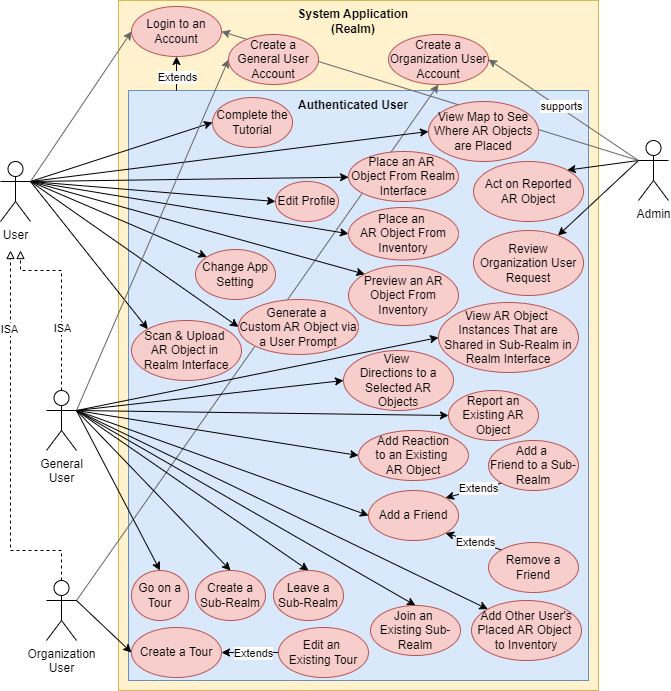
\includegraphics[scale=0.5]{use_cases.png}\\
    \textbf{Figure 1: Use Cases}
\end{center}

\begin{enumerate}[label=\textbf{UC\arabic*}]
    \item \label{uc:1} Complete the Tutorial \\
        \textbf{Actor}: \ref{def:user} \\
        \textbf{Pre-condition:} User has opened the app \\

        \textbf{Main Success Scenario:}
        \begin{enumerate}[label=\textbf{\arabic*.}]
            \item User creates an account (\ref{uc:23})
            \item System prompts user to complete the tutorial (\hyperref[ssub:tutorial]{TU-FR2})
            \item User indicates they would like to do the tutorial
            \item System opens the \textbf{Tutorial Interface}
            \item System provides directions to use a feature
            \item User tries the feature (\hyperref[ssub:tutorial]{TU-FR5})
            \item User goes to next feature when satisfied
            \item Repeat steps \textbf{5}-\textbf{7} for all major app features (\hyperref[ssub:tutorial]{TU-FR1})
            \item System prompts user to leave and end tutorial
            \item User ends tutorial (\hyperref[ssub:tutorial]{TU-FR3})
            \item System redirects to \textbf{Home Interface}
        \end{enumerate}

        \textbf{Secondary Scenarios:}
        \begin{itemize}
            \item[{\bf 1.1:}] User already has an account
            \begin{enumerate}[label=\textbf{\arabic*.}]
                \item User logs into account (\ref{uc:24})
                \item User navigates to \textbf{Help Interface} (\hyperref[ssub:tutorial]{TU-FR4})
                \item Go to step \textbf{2}
            \end{enumerate}
            \item[{\bf 10.1:}] User chooses to stay in sandbox environment
            \begin{enumerate}[label=\textbf{\arabic*.}]
                \item System closes prompt and allows user to use sandbox environment
                \item User indicates they want to leave tutorial
                \item Go to step \textbf{11}
            \end{enumerate}
        \end{itemize}
        \textbf{Success Postcondition:} The user has a general idea of how all the app’s major features work.

    \item \label{uc:2} Create a Tour \\
        \textbf{Actor}: \ref{def:org_user} \\
        \textbf{Pre-condition:} User is logged into the app \textbf{AND} User has navigated to the \textbf{Tour Management Interface} \\

        \textbf{Main Success Scenario:}
        \begin{enumerate}[label=\textbf{\arabic*.}]
            \item User selects the option to create a new tour
            \item System opens up a form for the user to add the following information about the tour (\hyperref[ssub:tour_management]{TM-FR4[1,2,5,6]}):
            \begin{enumerate}
                \item Name
                \item Description
                \item Price
                \item Relevant web link(s)
            \end{enumerate}
            \item User fills out the information
            \item System identifies no blank fields
            \item System gives the option to move on to the route configuration
            \item User goes to the route configuration
            \item System presents tour route configuration
            \item User configures tour area, route, and direction (\hyperref[ssub:tour_management]{TM-FR4[3]})
            \item System gives the option to move on to the inventory setup
            \item User goes to the inventory setup (\hyperref[ssub:tour_management]{TM-FR4[4]})
            \item System opens the \textbf{Inventory Interface}
            \item User scans and uploads a new \ref{def:ar_obj} (\ref{uc:5})
            \item User repeats step \textbf{12} until all desired \ref{def:ar_obj}s are uploaded
            \item User indicates they would like to move on to object placement
            \item System opens the \textbf{Realm Interface} and allows the user to place \ref{def:ar_obj}s and historical information popups in an isolated environment.
            \item User places down \ref{def:ar_obj} using the \textbf{Realm Interface} (\ref{uc:7})
            \item User repeats step \textbf{16} until all desired \ref{def:ar_obj}s are placed
            \item User indicates they would like to finish tour creation
            \item System gives the user the option create the tour as a draft or directly publish it (\hyperref[ssub:tour_management]{TM-FR2/TM-FR3})
            \item User selects direct publish option
            \item System uploads the tour data
            \item System makes the tour available to \ref{def:gen_user}
        \end{enumerate}

        \textbf{Secondary Scenarios:}
        \begin{itemize}
            \item[{\bf 4.1:}] System identifies some blank fields
            \begin{enumerate}[label=\textbf{\arabic*.}]
                \item System validates input to ensure all required fields are not empty
                \item System determines input passes validation
                \item Go to step \textbf{5}
            \end{enumerate}
            \item[{\bf 4.1.2:}] System determines input fails validation
            \begin{enumerate}[label=\textbf{\arabic*.}]
                \item Go to step \textbf{3}
            \end{enumerate}
            \item[{\bf 12.1:}] User does not have any \ref{def:ar_obj}s to scan
            \begin{enumerate}[label=\textbf{\arabic*.}]
                \item Go to step \textbf{14}
            \end{enumerate}
            \item[{\bf 20.1:}] User selects draft option
            \begin{enumerate}[label=\textbf{\arabic*.}]
                \item System uploads the tour data but does not make it available to \ref{def:gen_user}
                \item User decides at a later time to publish the draft tour
                \item Go to step \textbf{22}
            \end{enumerate}
        \end{itemize}
        \textbf{Success Postcondition:} One of the \ref{def:org_user} has a new tour linked to their organization

    \item \label{uc:3} Edit an existing Tour \\
        \textbf{Actor}: \ref{def:org_user} \\
        \textbf{Pre-condition:} User is logged into the app \textbf{AND} User has at least one tour connected to their organization \textbf{AND} User has navigated to the \textbf{Tour Management Interface} \\

        \textbf{Main Success Scenario:}
        \begin{enumerate}[label=\textbf{\arabic*.}]
            \item System provides a list of all tours connected to the user’s organization
            \item User selects one of the tours
            \item System shows the preview of the tour (\hyperref[ssub:tour_management]{TM-FR5})
            \item System provides the option to edit the tour (\hyperref[ssub:tour_management]{TM-FR6})
            \item User decides to edit the tour
            \item System opens up a form for the user to with the following information about the tour that may or not be populated (\hyperref[ssub:tour_management]{TM-FR4[1,2,5,6]}):
            \begin{enumerate}
                \item Name
                \item Description
                \item Price
                \item Relevant web link(s)
            \end{enumerate}
            \item User edits information as desired
            \item System identifies no blank fields
            \item System gives the option to move on to the route configuration
            \item User goes to the route configuration
            \item System presents tour route configuration
            \item User edits configuration of tour area, route, and direction as desired (\hyperref[ssub:tour_management]{TM-FR4[3]})
            \item System gives the option to move on to the inventory setup
            \item User goes to the inventory setup (\hyperref[ssub:tour_management]{TM-FR4[4]})
            \item System opens the \textbf{Inventory Interface}
            \item User scans and uploads a new \ref{def:ar_obj} (\ref{uc:5})
            \item User repeats step \textbf{12} until all desired \ref{def:ar_obj}s are uploaded
            \item User indicates they would like to move on to object placement
            \item System opens the \textbf{Realm Interface} and allows the user to place/edit \ref{def:ar_obj}s and historical information popups in an isolated environment.
            \item User edits \ref{def:ar_obj} using the \textbf{Realm Interface} (\ref{uc:7})
            \item User repeats step \textbf{16} until all desired \ref{def:ar_obj}s are edited
            \item User indicates they would like to finish tour editing
            \item System gives the user the option to save the edited tour as a draft or directly publish it (\hyperref[ssub:tour_management]{TM-FR2/TM-FR3})
            \item User selects direct publish option
            \item System uploads the updated tour data
            \item System makes the updated tour available to \ref{def:gen_user}
        \end{enumerate}

        \textbf{Secondary Scenarios:}
        \begin{itemize}
            \item[{\bf 5.1:}] User decides not to edit the tour
            \begin{enumerate}[label=\textbf{\arabic*.}]
                \item System goes back to the \textbf{Tour Management Interface}
            \end{enumerate}
            \item[{\bf 8.1:}] System identifies some blank fields
            \begin{enumerate}[label=\textbf{\arabic*.}]
                \item System validates input to ensure all required fields are not empty
                \item System determines input passes validation
                \item Go to step \textbf{9}
            \end{enumerate}
            \item[{\bf 16.1:}] User decides not to scan and upload any new \ref{def:ar_obj}s
            \begin{enumerate}[label=\textbf{\arabic*.}]
                \item Go to step \textbf{18}
            \end{enumerate}
            \item[{\bf 20.1:}] User places down new \ref{def:ar_obj} using the \textbf{Realm Interface}
            \begin{enumerate}[label=\textbf{\arabic*.}]
                \item User repeats step \textbf{20.1} until all desired \ref{def:ar_obj}s are placed
            \end{enumerate}
            \item[{\bf 24.1:}] User selects draft option
            \begin{enumerate}[label=\textbf{\arabic*.}]
                \item System uploads the updated tour data but does not make it available to \ref{def:gen_user}
                \item User decides at a later time to publish the draft of the updated tour
                \item Go to step \textbf{26}
            \end{enumerate}
        \end{itemize}
        \textbf{Success Postcondition:} One of the \ref{def:org_user} has edited an existing tour linked to their organization

    \item \label{uc:4} Go on a tour \\
        \textbf{Actor}: \ref{def:gen_user} \\
        \textbf{Pre-condition:} User is logged into the app \\

        \textbf{Main Success Scenario:}
        \begin{enumerate}[label=\textbf{\arabic*.}]
            \item User navigates to the \textbf{Tour Interface}
            \item System displays a list of all tours
            \item User selects a tour (\hyperref[ssub:touring]{TR-FR2.1})
            \item System opens up the preview of the selected tour (\hyperref[ssub:touring]{TR-FR3})
            \item System also provides the option to take the tour
            \item User reviews details of the tour
            \item User decides to go on the tour
            \item System opens a modified version of the \textbf{Realm Interface} in an isolated environment that does not allow them to place any objects or modify existing objects (\hyperref[ssub:touring]{TR-FR4.2})
            \item System shows the intended direction of travel
            \item User walks to the highlighted \ref{def:ar_obj} of interest
            \item System acknowledges when the user makes it to the \ref{def:ar_obj}
            \item System provides historical information regarding \ref{def:ar_obj}
            \item System updates the target to be the next \ref{def:ar_obj}
            \item Repeat steps \textbf{10}-\textbf{13} for every \ref{def:ar_obj}
            \item System indicates that the tour has been completed
            \item System provides metrics for time taken and distance traveled
            \item System prompts user to leave tour
            \item User leaves tour
            \item System goes back to the tour list
        \end{enumerate}

        \textbf{Secondary Scenarios:}
        \begin{itemize}
            \item[{\bf 1.1:}] System pushes a notification to the user when they are in the proximity of a tour (\hyperref[ssub:touring]{TR-FR2.2})
            \begin{enumerate}[label=\textbf{\arabic*.}]
                \item System opens up the \textbf{Tour Interface}
                \item Go to step \textbf{4}
            \end{enumerate}
            \item[{\bf 1.2:}] User scans a tour QR code in camera app (\hyperref[ssub:touring]{TR-FR2.3})
            \begin{enumerate}[label=\textbf{\arabic*.}]
                \item System opens up the \textbf{Tour Interface}
                \item Go to step \textbf{4}
            \end{enumerate}
            \item[{\bf 7.1:}] User decides not to go on the tour
            \begin{enumerate}[label=\textbf{\arabic*.}]
                \item Go to step \textbf{19}
            \end{enumerate}
            \item[{\bf 10.1:}] User indicates they want to open the map
            \begin{enumerate}[label=\textbf{\arabic*.}]
                \item System opens up the \textbf{Map} view of the tour (\hyperref[ssub:touring]{TR-FR4.2})
                \item System shows the user’s current location
                \item System shows the indented route, direction and boundaries of the tour
                \item System marks the location of \ref{def:ar_obj}s
                \item User views the map
                \item User closes the map
                \item Go to step \textbf{9}
            \end{enumerate}
            \item[{\bf 14.1:}] User does not want to go to all \ref{def:ar_obj}s
            \begin{enumerate}[label=\textbf{\arabic*.}]
                \item User indicates they wish to exit the tour
                \item Go to step \textbf{19}
            \end{enumerate}
            \item[{\bf 18.1:}] User does not leave tour
            \begin{enumerate}[label=\textbf{\arabic*.}]
                \item System removes target object and allows user to explore \ref{def:ar_obj}s in the isolated environment
                \item User eventually decides to exit the tour
                \item Go to step \textbf{19}
            \end{enumerate}
        \end{itemize}
        \textbf{Success Postcondition:} One of the \ref{def:gen_user} has completed a tour

        \item \label{uc:5} Scan and upload \ref{def:ar_obj} to the user inventory \\
        \textbf{Actor}: \ref{def:gen_user} \\
        \textbf{Pre-condition:} User has an account on the application \textbf{AND} is logged into the application \textbf{AND} navigates to the Realm display \\

        \textbf{Main Success Scenario:}
        \begin{enumerate}[label=\textbf{\arabic*.}]
            \item System displays Realm screen to user
            \item User selects control to scan and create an \ref{def:ar_obj}
            \item System presents user with the option to scan a 2D or 3D \ref{def:ar_obj}
            \item User selects one of the provided options
            \begin{enumerate}[label=(\alph*)]
                \item User selects 2D \ref{def:ar_obj} option
                \item User selects 3D \ref{def:ar_obj} option
            \end{enumerate}
            \item System displays a scanning interface
            \item User performs motions to scan the targeted object
            \item System provides a render for the scanned portion (happens concurrently with step \textbf{6})
            \item User selects the option to confirm that the scanning process is complete
            \item System navigates user to an editor with the complete render of the target entity
            \item User performs actions to edit the render to meet their needs
            \begin{enumerate}[label=(\alph*)]
                \item User removes unneeded parts of the render
                \item User changes the colour of selected portions
            \end{enumerate}
            \item System applies the changes to the \ref{def:ar_obj} intended by the user
            \item User confirms that the editing process is completed
            \item System receives the user confirmation and provides a preview of the final \ref{def:ar_obj} with the options to discard or add it to their inventory
            \item User selects what they would want to do with the new \ref{def:ar_obj}
            \begin{enumerate}[label=(\alph*)]
                \item User returns to the editing interface for further customization (Go to step \textbf{10})
                \item User selects control to add the object to their inventory
                \item User wants to discard the object (Go to Secondary Scenario 2)
            \end{enumerate}
            \item System adds the new \ref{def:ar_obj} to the User's inventory and notifies the User about adding the object to their inventory
            \item System returns to the Realm screen
        \end{enumerate}

        \textbf{Secondary Scenarios:}
        \begin{itemize}
            \item[\textbf{\textbf{(3.1, 5.1)}}] User cancels scanning process
            \begin{enumerate}[label=\textbf{\arabic*.}]
                \item Main scenario steps \textit{1-3 or 1-5}
                \item User selects option to cancel the scanning process
                \item System receives User's request to cancel scanning process and returns to the Realm screen
            \end{enumerate}

            \item[9.1] User discards the scanned \ref{def:ar_obj}
            \begin{enumerate}[label=\textbf{\arabic*.}]
                \item Main scenario steps \textit{1-9}
                \item User selects option to discard the scanned object
                \item System receives User's request and presents confirmation prompt for discarding object
                \item User interacts with confirmation prompt
                \begin{enumerate}[label=(\alph*)]
                    \item User selects to discard object
                    \item User selects to not discard object (Go back to Main scenario step \textbf{13})
                \end{enumerate}
                \item System receives User response and deletes object and returns to the Realm screen
            \end{enumerate}

        \end{itemize}
        \textbf{Success Postcondition:} The User can view the new object in their inventory

        \item \label{uc:6} Generate a custom \ref{def:ar_obj} via a user prompt \\
        \textbf{Actor}: \ref{def:gen_user} \\
        \textbf{Pre-condition:} User has an account on the application \textbf{AND} is logged in to the app \textbf{AND} has navigated to the \textbf{Realm Interface} \\

        \textbf{Main Success Scenario:}
        \begin{enumerate}[label=\textbf{\arabic*.}]
            \item User is present in the Realm Interface and performs actions to navigate to the object prompt generation interface
            \item System presents the object prompt generation interface
            \item User enters their desired prompt and confirms that the prompt is complete
            \item System checks the prompt for profanity
            \begin{enumerate}[label=(\alph*)]
                \item If the prompt contains profanity, system notifies user that the prompt is invalid due to profanity and requests the user to reenter their prompt (Go to step \textbf{2})
                \item If the prompt does not contain profanity, system accepts the prompt and generates objects
            \end{enumerate}
            \item User selects from an array of objects provided by the system
            \item System provides the options to \textbf{preview the object}, \textbf{add it to user inventory} and \textbf{place object in the Realm Interface}
            \item User selects one of the options
            \begin{enumerate}[label=(\alph*)]
                \item User selects the options to preview the object
                \item User selects to add object to their inventory
                \item User selects option to place object in the Realm Interface
            \end{enumerate}
            \item System performs the action selected by the user
            \begin{enumerate}[label=(\alph*)]
                \item User selects option to preview object
                \begin{enumerate}
                    \item System opens the \ref{def:ar_obj} in the Preview Interface
                    \item User performs actions on the \ref{def:ar_obj}
                    \begin{itemize}
                        \item User rotates the object to view different angles
                        \item User zooms in and out to view object details
                    \end{itemize}
                    \item System provides the view of the \ref{def:ar_obj} according to the User's performed actions
                \end{enumerate}
                \item User selects option to add object to inventory
                \begin{enumerate}
                    \item System adds object to user inventory
                \end{enumerate}
                \item User selects option to place object in the Realm space (Go to \ref{uc:7} Main Success Scenario)
            \end{enumerate}
        \end{enumerate}

        \textbf{Secondary Scenarios:}
        \begin{itemize}
            \item[\textbf{(2.1, 4(b).1)}] User cancels the \ref{def:ar_obj} generation
            \begin{enumerate}[label=\textbf{\arabic*.}]
                \item Main scenario steps \textit{1-2 or 1-4(b)}
                \item User selects control to cancel object generation via prompt
                \item System receives user request and returns to the Realm interface
            \end{enumerate}

            \item[\textbf{(2.1, 4(a).1)}] User reenters prompt due to presence of profanity
            \begin{enumerate}[label=\textbf{\arabic*.}]
                \item Main scenario steps \textit{1-2 or 1-4(a)}
                \item User is notified of profanity in the prompt and reenters their prompt
                \item Go to Main scenario step 4
                \item Continues Main Scenario from step 5
            \end{enumerate}

            \item[\textbf{(2.1, 4(b).1)}] User reenters prompt for a different variation
            \begin{enumerate}[label=\textbf{\arabic*.}]
                \item Main scenario steps \textit{1-2 or 1-4(b)}
                \item User reenters their prompt
                \item System validates user prompt (Go to Main scenario step \textbf{4})
                \item Continues Main Scenario from step \textbf{5}
            \end{enumerate}

        \end{itemize}
        \textbf{Success Postcondition:} The User can view the new object in their inventory

        \item \label{uc:9} Preview AR objects from the Inventory \\
        \textbf{Actor}: \ref{def:gen_user} \\
        \textbf{Pre-condition:} User has an account on the system \textbf{AND} is logged into the system \\

        \textbf{Main Success Scenario:}
        \begin{enumerate}[label=\textbf{\arabic*.}]
            \item User navigates to their profile view
            \item System presents the User's profile and inventory
            \item User selects controls to view their entire inventory
            \item System provides complete view of the inventory
            \item User selects an \ref{def:ar_obj} they would like to view
            \item System provides the option to preview the \ref{def:ar_obj}
            \item User selects the option to preview the \ref{def:ar_obj}
            \item System opens the \ref{def:ar_obj} in the Preview Interface
            \item User performs actions on the \ref{def:ar_obj}
            \begin{enumerate}[label=(\alph*)]
                \item User rotates the object to view different angles
                \item User zooms in and out to view object details
            \end{enumerate}
            \item System provides the view of the \ref{def:ar_obj} according to the User's performed actions
        \end{enumerate}

        \textbf{Secondary Scenarios:}
        N/A

        \textbf{Success Postcondition:} User is able to view an \ref{def:ar_obj} in their inventory from different angles

        \item \label{uc:11} Check the map to see where objects are placed in the world \\
        \textbf{Actor}: \ref{def:gen_user} \\
        \textbf{Pre-condition:} User has an account on the application \textbf{AND} is logged in to the app \\

        \textbf{Main Success Scenario:}
        \begin{enumerate}[label=\textbf{\arabic*.}]
            \item User performs actions to navigate to the Map view
            \item System presents the Maps Interface
            \item User observes location markers with the count of the objects and selects a marker
            \item System shows information and options for the marker
            \begin{enumerate}[label=(\alph*)]
                \item System displays number of visits to the marker, the number of objects available and the area covered by the marker
                \item System provides the options to receive directions for the selected marker (Go to \ref{uc:12})
            \end{enumerate}
        \end{enumerate}

        \textbf{Secondary Scenarios:}
        N/A

        \textbf{Success Postcondition:} User is able to view cluster of objects in a confined area on the Maps Interface

    \item \label{uc:12}  Provide directions to a selected group of objects \\
        \textbf{Actor}: \ref{def:gen_user} \\
        \textbf{Pre-condition:} User has an account on the application \textbf{AND} is logged in to the app \textbf{AND} is present on the Maps Interface \\

        \textbf{Main Success Scenario:}
        \begin{enumerate}[label=\textbf{\arabic*.}]
            \item User selects a location marker on the Map Interface
            \item System shows information about the marker (see \ref{uc:11} Main scenario step \textit{4(a)}) and the option to provide directions for the marker
            \item User selects the option to get directions for the location markers
            \item System provides a set of instructions to direct the user to the marker
            \item User views the instructions and follows the directions provided
            \item System tracks User location to check if they have arrived at the marker location (happens concurrently with step 5)
            \item User arrives at the selected marker
            \item System is informed that the user has arrived at the marker location (based on device location) and notifies the User of their arrival
        \end{enumerate}

        \textbf{Secondary Scenarios:}
        \begin{itemize}
            \item[{\textbf{6.1}}] User ends navigation to marker before reaching the marker
            \begin{enumerate}[label=\textbf{\arabic*.}]
                \item Main Sceanrio step \textit{1-6}
                \item User selects option to end navigation to the marker
                \item System provides a confirmation prompt for ending the navigation
                \item User responds to the confirmation prompt
                \begin{enumerate}[label=(\alph*)]
                    \item User selects option to confirm terminating navigation
                    \item User selects option to deny terminating the navigation and continues navigation (Go to Main scenario step \textit{5})
                \end{enumerate}
                \item System ends navigation and returns to the Map Interface
            \end{enumerate}
        \end{itemize}
        \textbf{Success Postcondition:} The User is provided the directions to their chosen marker and have arrived at the marker location

    \item \label{uc:26}  Act on reported \ref{def:ar_obj} \\
        \textbf{Actor}: \ref{def:admin} \\
        \textbf{Pre-condition:} Admin is logged into the app \textbf{AND} Admin has navigated to the \textbf{Admin Interface} \\

        \textbf{Main Success Scenario:}
        \begin{enumerate}[label=\textbf{\arabic*.}]
            \item Admin navigates to the “AR Object Reports” panel (\hyperref[ssub:admin_interface]{AI-FR2.1})
            \item System shows a list of app \ref{def:ar_obj}s that have been reported
            \item Admin selects an object
            \item System gives more detailed information of \ref{def:ar_obj} and allows Admin to open an \ref{def:ar_obj} inventory preview (\hyperref[ssub:inventory]{IV-FR6})
            \item System also provides decision options on whether to keep the object or remove it
            \item Admin opens \ref{def:ar_obj} preview
            \item System shows preview of \ref{def:ar_obj}
            \item Admin views \ref{def:ar_obj} preview
            \item Admin closes \ref{def:ar_obj} preview
            \item System once again shows the object detailed information and decision options
            \item Admin reviews the information and decides to keep the \ref{def:ar_obj}
            \item System keeps \ref{def:ar_obj}
            \item System removes user report of \ref{def:ar_obj}
            \item System brings admin back to “AR Object Reports” panel
        \end{enumerate}

        \textbf{Secondary Scenarios:}
        \begin{itemize}
            \item[{\bf 5.1:}] Admin does not open \ref{def:ar_obj} preview
            \begin{enumerate}[label=\textbf{\arabic*.}]
                \item Go to step \textbf{11}
            \end{enumerate}
            \item[{\bf 11.1:}] Admin reviews the information and decides to remove the object
            \begin{enumerate}[label=\textbf{\arabic*.}]
                \item System removes object
                \item Go to step \textbf{13}
            \end{enumerate}
        \end{itemize}
        \textbf{Success Postcondition:} An \ref{def:ar_obj} report is resolved (\ref{def:ar_obj} is kept or removed)

    \item \label{uc:27}  Act on reported \ref{def:ar_obj} \\
        \textbf{Actor}: \ref{def:admin} \\
        \textbf{Pre-condition:} Admin is logged into the app \textbf{AND} Admin has navigated to the \textbf{Admin Interface} \\

        \textbf{Main Success Scenario:}
        \begin{enumerate}[label=\textbf{\arabic*.}]
            \item Admin navigates to the “Organization User Requests” panel (\hyperref[ssub:admin_interface]{AI-FR2.2})
            \item System shows a list of \ref{def:org_user} requests
            \item Admin selects a request
            \item System gives more details about a request
            \item System also provides decision options on whether to accept or decline a request
            \item Admin reviews information and approves the request
            \item System activates the user as one of the \ref{def:org_user}
            \item System notifies the user that their request has been approved
            \item System removes organization user request
            \item System brings admin back to “Organization User Requests” panel
        \end{enumerate}

        \textbf{Secondary Scenarios:}
        \begin{itemize}
            \item[{\bf 6.1:}] Admin reviews information and denies the request
            \begin{enumerate}[label=\textbf{\arabic*.}]
                \item System notifies the user that their request has been denied and gives a reason why
                \item Go to step \textbf{9}
            \end{enumerate}
        \end{itemize}
        \textbf{Success Postcondition:} An \ref{def:org_user} account request is resolved (approved or denied).

\end{enumerate}

\subsection{Quality of Service}

\wss{This section states additional, quality-related property requirements that the functional effects of the software should present.}
\subsubsection{Performance}

\wss{If there are performance requirements for the product under various circumstances, state them here and explain their rationale, to help the developers understand the intent and make suitable design choices. Specify the timing relationships for real time systems. Make such requirements as specific as possible. You may need to state performance requirements for individual functional requirements or features.}

\subsubsection{Security}

\wss{Specify any requirements regarding security or privacy issues surrounding use of the product or protection of the data used or created by the product. Define any user identity authentication requirements. Refer to any external policies or regulations containing security issues that affect the product. Define any security or privacy certifications that must be satisfied.}

\subsubsection{Reliability}

\wss{Specify the factors required to establish the required reliability of the software system at time of delivery.}

\subsubsection{Availability}

\wss{Specify the factors required to guarantee a defined availability level for the entire system such as checkpoint, recovery, and restart.}

\subsection{Compliance}
\label{sub:compliance}

\wss{Specify the requirements derived from existing standards or regulations, including:
    \begin{itemize}
        \item Report format
        \item Data naming
        \item Accounting procedures
        \item Audit tracing
    \end{itemize}
}

\wss{For example, this could specify the requirement for software to trace processing activity. Such traces are needed for some applications to meet minimum regulatory or financial standards. An audit trace requirement may, for example, state that all changes to a payroll database shall be recorded in a trace file with before and after values.}

\begin{enumerate}[align=left, label=\textbf{CO\arabic*.}]
    \item The project shall comply with the \emph{Personal Information and Electronic Documents Act} (PIPEDA).\\
    {\bf Rationale:} The Government of Canada requires all companies to follow certain rules regarding the collection, use, and dissemination of personal user information \cite{PIPEDA}.
    \item The project shall keep records of all in-app purchases and ad revenue for the purposes of yearly tax filing for the period of six years.\\
    {\bf Rationale:} Corporate taxes must be filed every year and both streams of app income will need to be reported. Businesses must keep records going back six years in the event of an audit \cite{6Year}.
    \item The app shall comply with the \emph{Google Play} developer policy.\\
    {\bf Rationale:} All apps published through \emph{Google Play} must first be reviewed by Google for compliance with the developer policy published on their website \cite{GooglePlay}.
    \item The app shall comply with \emph{App Store} review guidelines.\\
    {\bf Rationale:} For an app to be approved for dissemination on the \emph{App Store}, the app must be reviewed and approved by Apple in accordance with the acceptance criteria published on their website \cite{AppStore}.
\end{enumerate}

\subsection{Design and Implementation}

\subsubsection{Installation}
\label{ssub:installation}

\wss{Constraints to ensure that the software-to-be will run smoothly on the target implementation platform.}

\begin{enumerate}[align=left, label=\textbf{DI-I\arabic*.}]
    \item The app shall be installable on \emph{Android} and \emph{iOS} devices from their respective app stores.\\
    {\bf Rationale:} Users are accustomed to downloading their apps from their device app store and should not be required to navigate to a 3rd party app store. They also should not have to change OS settings in order to download the app.
    \item The app shall not require any additional installation steps beyond those required from within the target device app store.\\
    {\bf Rationale:} Users may be dissuaded from downloading the app if the installation process is too cumbersome compared to other apps.
\end{enumerate}

\subsubsection{Distribution}
\label{ssub:distribution}

\wss{Constraints on software components to fit the geographically distributed structure of the host organization, the distribution of data to be processed, or the distribution of devices to be controlled.}

\begin{enumerate}[align=left, label=\textbf{DI-D\arabic*.}]
    \item The app shall be distributed on any mobile devices running iOS 16.0+ or Android 12+\\
    {\bf Rationale:} The app should be available to as many people as possible while at the same time making the development easier by not having to keep old operating system versions supported. Versions should be supported for at least a couple years.
    \item The app shall be available in Canada and the USA.\\
    {\bf Rationale:} Due to legal considerations in different countries, the focus for this app should be the country this project is based out of, Canada, and the USA since they have a larger population with similar laws.
    \item The app shall have a recommended age requirement of 16+.\\
    {\bf Rationale:} Users may be exposed to content not suitable for really young kids so an age requirement should be recommended.
    \item The system shall store all user data within North America.\\
    {\bf Rationale:} Data should be located in a jurisdiction close to home and in a reputable country to reduce privacy concerns of foreign state actors viewing user data.
\end{enumerate}

\subsubsection{Maintainability}

\wss{Specify attributes of software that relate to the ease of maintenance of the software itself. These may include requirements for certain modularity, interfaces, or complexity limitation. Requirements should not be placed here just because they are thought to be good design practices.}

\subsubsection{Reusability}

\subsubsection{Portability}
\label{ssub:portability}

\wss{Specify attributes of software that relate to the ease of porting the software to other host machines and/or operating systems.}

\begin{enumerate}[align=left, label=\textbf{DI-P\arabic*.}]
    \item The app shall be developed using a cross-platform mobile platform that can build iOS and Android applications\\
    {\bf Rationale:} To reach as many potential users as possible, the app should be available on the two major mobile operating systems.
    \item The app shall have a common codebase that only differs in configuration files for different target operating systems.\\
    {\bf Rationale:} For ease of development on the different mobile operating systems, there should be no extra consideration for the differences between native app implementations that are not handled by the cross-platform framework.
\end{enumerate}

\subsubsection{Cost}

\wss{Specify monetary cost of the software product.}

\subsubsection{Deadline}

\wss{Specify schedule for delivery of the software product.}

\subsubsection{Proof of Concept}

\section{Verification}

\wss{This section provides the verification approaches and methods planned to qualify the software. The information items for verification are recommended to be given in a parallel manner with the requirement items in Section 3. The purpose of the verification process is to provide objective evidence that a system or system element fulfills its specified requirements and characteristics.}

\section{Appendixes}

\subsection{Activity Diagrams}
\label{sub:activity_diagrams}

\begin{center}
    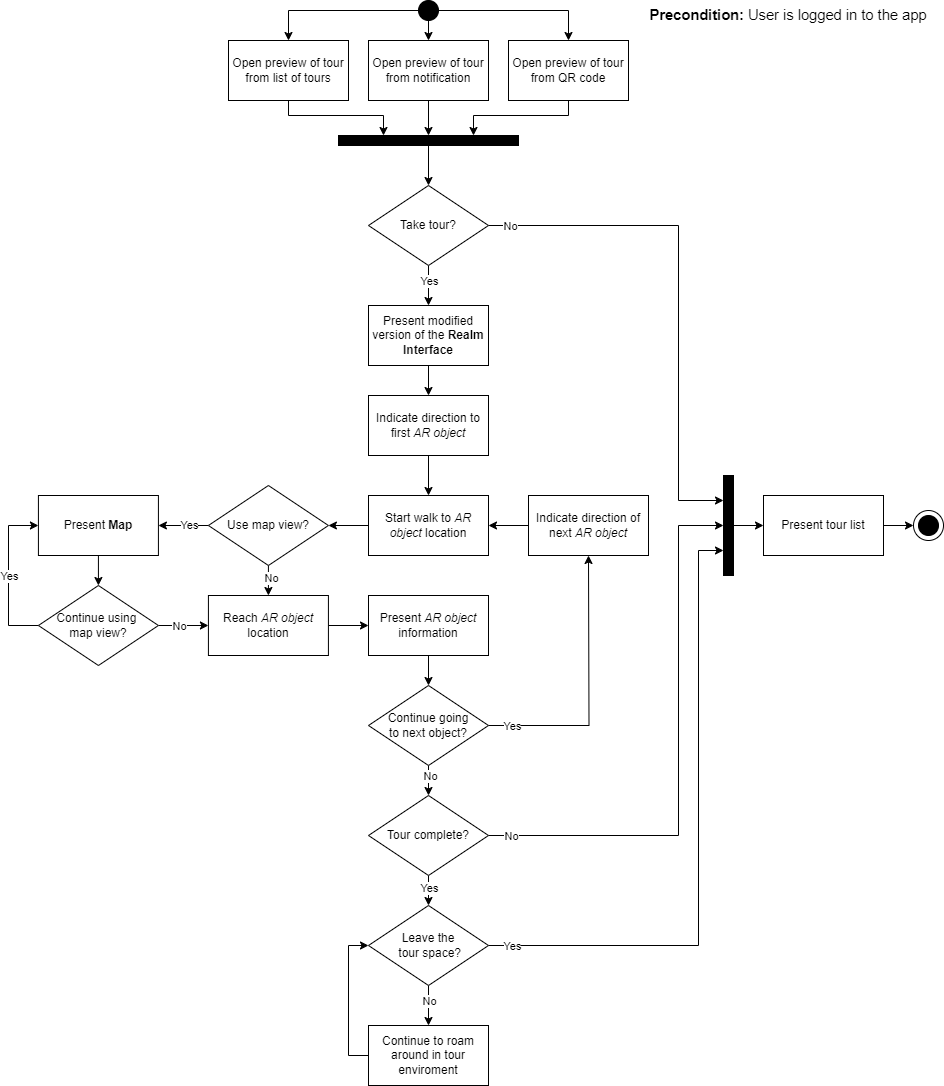
\includegraphics[scale=0.4]{SequenceDiagrams/UC4.png}\\
    \textbf{Figure 2: UC4}
\end{center}

\subsection{Reflection}

The information in this section will be used to evaluate the team members on the
graduate attribute of Lifelong Learning.  Please answer the following questions:

\begin{enumerate}
    \item What knowledge and skills will the team collectively need to acquire to
          successfully complete this capstone project?  Examples of possible knowledge
          to acquire include domain specific knowledge from the domain of your
          application, or software engineering knowledge, mechatronics knowledge or
          computer science knowledge.  Skills may be related to technology, or writing,
          or presentation, or team management, etc.  You should look to identify at
          least one item for each team member.
    \item For each of the knowledge areas and skills identified in the previous
          question, what are at least two approaches to acquiring the knowledge or
          mastering the skill?  Of the identified approaches, which will each team
          member pursue, and why did they make this choice?
\end{enumerate}


\end{document}
